% Este archivo es parte de la presentación de libWiiEsp, protegida bajo la 
% licencia GFDL. Copyright (C) 2011 Ezequiel Vázquez de la Calle

% -*-presentacion.tex-*-

\documentclass{beamer}
\usepackage[utf8x]{inputenc}
\usepackage[spanish]{babel}
\usepackage{graphicx}
\usepackage{listings}
\usepackage{fancyvrb}
\usepackage{color}
\usetheme{Warsaw}
\setbeamertemplate{headline}[default]
\setlength\fboxsep{0pt}
\setlength\fboxrule{0.1pt}
\graphicspath{{./imagenes/}}

\title[LibWiiEsp]{LibWiiEsp: Biblioteca libre de desarrollo de videojuegos para Nintendo Wii}
\author[Ezequiel Vázquez de la Calle]{Ezequiel Vázquez de la Calle \\ Codirectores: \\ Manuel Palomo Duarte \\ Antonio García Domínguez}
\date{}
\institute[UCA]

\begin{document}
% Primera pagina
\def\newblock{\hskip .11em plus .33em minus .07em}

\begin{frame}[fragile]{}
    \titlepage 
    \begin{picture}(0,0)
        \put(130,-10){
\includegraphics[scale=0.1]{logo_uca.png}}
    \end{picture}
\end{frame}
%-------------------------

\normalsize

% Mostrar indice antes de la secciones
\AtBeginSection[] {
  \begin{frame}{Índice}
    \tableofcontents[currentsection]
  \end{frame}} 
%-------------------------

% Introducción
% Este archivo es parte de la memoria de libWiiEsp, protegida bajo la 
% licencia GFDL. Puede encontrar una copia de la licencia en el archivo fdl-1.3.tex

% Fuente tomada de la plantilla LaTeX para la realización de Proyectos Final 
% de Carrera de Pablo Recio Quijano.

% Copyright (C) 2009 Pablo Recio Quijano
% Copyright (C) 2011 Ezequiel Vázquez de la Calle

% -*-introduccion.tex-*-

Actualmente, el sector de los videojuegos está en alza, llegando en algunos países europeos a facturar más que la industria cinematográfica. A lo largo de los años, han visto la luz multitud de sistemas especializados en la ejecución de estas aplicaciones software de entretenimiento, las videoconsolas. Sin embargo, es común en este mundillo que los fabricantes no permitan la ejecución de código no firmado por ellos en dichas plataformas. Gracias a la labor de muchas personas a lo largo y ancho del planeta, se ha hecho posible el desarrollo de software casero en algunas videoconsolas (por ejemplo, en la \emph{Sony PlayStation 3}, o en la \emph{Nintendo Wii}). Generalmente, las herramientas para construir y ejecutar este software suele ser de muy bajo nivel, y, en muchas ocasiones, de código cerrado y sin documentación técnica alguna disponible, por lo que se hace patente la necesidad de facilitar al gran público herramientas libres que cubran las posibilidades de desarrollo en estas videoconsolas.\\

A continuación, se describe de forma general el contenido del proyecto y de esta memoria.

\section{Objetivos}

Los objetivos de este proyecto son varios, entre los cuales destacan especialmente el afán de conocimiento sobre el funcionamiento de una videoconsola (en este caso concreto, la Nintendo Wii), la puesta en práctica de los conocimientos adquiridos durante las asignaturas de la titulación de \emph{Ingeniería Técnica en Informática de Gestión}, la profundización en los métodos de programación de videojuegos de dos dimensiones (ampliando lo aprendido en la asignatura \emph{Diseño de Videojuegos}), y el deseo de aportar una herramienta completa, libre, de alto nivel y documentada en español para el desarrollo de videojuegos en la plataforma Nintendo Wii.\\

La lista completa de objetivos que se persiguen con la realización del proyecto son los siguientes:

\begin{itemize}
\item \textbf{Aportar una herramienta completa de desarrollo de videojuegos 2D en Wii}: se pretende ofrecer al mundo del \emph{software libre} una forma de desarrollar videojuegos en dos dimensiones para la consola Nintendo Wii, que resulte sencilla de utilizar, pero que a su vez permita construir juegos completos.
\item \textbf{Proporcionar una visión general sobre el funcionamiento de la consola}: una videoconsola no es más que un ordenador dedicado exclusivamente a la ejecución de videojuegos; sin embargo, existen numerosas diferencias en el desarrollo de un programa para una consola respecto a hacerlo para un ordenador personal. Si bien no se desea profundizar al máximo en este asunto, sí se quiere aportar una idea más o menos completa del cambio que supone elegir una plataforma de desarrollo u otra.
\item \textbf{Ofrecer una documentación completa en español}: actualmente, existen pocas herramientas de desarrollo libres para Nintendo Wii, y las que hay son de muy bajo nivel, además de estar poco o nada documentadas. Con este proyecto se busca proporcionar una documentación completa, detallada y en español, de tal manera que cualquier persona con ciertos conocimientos sobre programación de videojuegos y orientación a objetos pueda desarrollar fácilmente un videojuego para la videoconsola.
\item \textbf{Desarrollar tres juegos de ejemplo}: la mejor manera de dominar una herramienta software es practicar con ella, pero siempre es conveniente tener un producto acabado que sirva de referencia. En este proyecto se quiere aportar tres juegos, totalmente funcionales y relativamente completos, que ilustren los resultados hasta los que se puede llegar con la biblioteca \programa{LibWiiEsp}.
\subitem \textbf{Arkanoid}: clon del clásico de \emph{Taito}, en el que el jugador debe destruir ladrillos, golpeándolos con una pelota que rebota en las paredes del escenario, y debe evitar también que la pelota caiga hacia la zona inferior de la pantalla.
\subitem \textbf{Duck Hunt}: basado en el clásico de \emph{Nintendo}. En lugar del comportamiento del videojuego de 1984, en éste participan dos jugadores a la vez. El objetivo de una partida consistirá en ser el primero de los dos en abatir un número concreto de patos.
\subitem \textbf{Wii Pang}: clon del clásico \programa{Pang} de \emph{Mitchel Co.} de 1989. El jugador controla a un personaje que debe evitar ser aplastado por unas pompas de colores que rebotan en el escenario del juego. Este personaje lanza ganchos verticales para romper las pompas en otras dos más pequeñas, que se vuelven a dividir en dos cuando reciben otro impacto sucesivamente hasta desaparecer al llegar a su tamaño más pequeño.
\end{itemize}

\section{Alcance}

Este proyecto pretende cubrir la escasez de herramientas libres que permiten desarrollar videojuegos en dos dimensiones para la consola Nintendo Wii, aportando una biblioteca con la que resulte fácil, pero a la vez eficiente, la construcción de juegos para esta plataforma. También proporciona una documentación útil y completa, enteramente en español, en contraposición a la poca información disponible sobre este tema, y que en general sólo puede encontrarse en inglés.

\subsection{Identificación del producto}

El producto resultante de este proyecto es \programa{LibWiiEsp}, una biblioteca libre y completa, pensada para hacer posible, de una forma sencilla y eficaz, el desarrollo de videojuegos libres en dos dimensiones para Nintendo Wii.

\subsection{Funcionalidades}

Esta biblioteca, escrita en C++ \cite{abur01} y publicada bajo licencia GPLv3, proporciona una interfaz que permite interactuar con los mandos, el sistema gráfico, el sistema de sonido y el lector de tarjetas SD de la consola. Además, incluye un \programa{parser} de XML sencillo pero efectivo, un sistema de soporte de internacionalización basado en ficheros XML, un sistema de gestión de contenido multimedia (imágenes, efectos de sonido, pistas de música y fuentes de texto), registro de eventos del sistema (\emph{logging}), creación de animaciones a partir de una imagen organizada en rejilla (\emph{spritesheet}) y un módulo de detección de colisiones basado en figuras planas fácilmente ampliable.\\

Como último punto a destacar, \programa{LibWiiEsp} incluye tres clases abstractas pensadas para ser utilizadas como plantillas para la creación de actores, niveles y la clase principal del videojuego (en la que se controla el bucle principal). La plantilla para niveles permite crear éstos con la herramienta libre Tiled \cite{website:tiled}, de tal manera que se facilita la creación de escenarios nuevos una vez terminada la programación del juego.\\

Parte importante del proyecto es también la documentación, que incluye un manual de instalación del entorno y de uso de las plantillas, y un manual de referencia completo.\\

A pesar de que es posible utilizar \programa{LibWiiEsp} en sistemas \programa{Windows}, \programa{GNU/Linux} y \programa{Mac}, la documentación sólo contempla los sistemas \programa{GNU/Linux}. Además, cabe destacar que el proceso de aprendizaje a la hora de utilizar la biblioteca requiere un esfuerzo moderado en un principio, debido al deseo de cubrir todos los aspectos del desarrollo de un videojuego en dos dimensiones.

\subsection{Aplicaciones del software}

El principal beneficio que aporta \programa{LibWiiEsp} es el de proporcionar, a cualquier persona con conocimientos de C++ y orientación a objetos, la posibilidad de desarrollar videojuegos en dos dimensiones en la plataforma Nintendo Wii.\\

El aporte de documentación completamente en español y el empleo de técnicas de programación adquiridas durante el transcurso de la titulación de \emph{Ingeniería Técnica en Informática de Gestión}, unido a la sencillez que aporta a la hora del desarrollo, hacen que el producto sea ideal para aprender y poner en práctica los procesos implicados en el diseño y creación de un videojuego en dos dimensiones.\\

Por otra parte, la evolución natural de una herramienta como es \programa{LibWiiEsp} podría producir la creación de una comunidad hispana de desarrolladores de videojuegos libres para la consola de Nintendo; si bien este hecho puede considerarse algo ambicioso, es una posibilidad a contemplar.

\section{Definiciones, abreviaturas y acrónimos}

\begin{itemize}
\item \textbf{Scener}: persona que ha colaborado en la obtención de información sobre cómo ejecutar código casero en un sistema cerrado, como una videoconsola o un \emph{smartphone}. Un \emph{scener} suele desarrollar aplicaciones libres basadas en la posibilidad de ejecución de software no firmado digitalmente por el fabricante (por ejemplo, un equipo de cuatro personas ha desarrollado un reproductor multimedia para la Nintendo Wii).
\item \textbf{Libogc}: biblioteca de muy bajo nivel, escrita en C, y desarrollada por varios \emph{sceners}. Brinda acceso a todo el hardware de la consola, pero es bastante compleja de utilizar.
\item \textbf{Spritesheet}: imagen o textura, organizada en rejilla, en la que cada recuadro de la rejilla contiene un fotograma de una animación.
\item \textbf{Textura organizada en \emph{tiles}}: una textura se representa en memoria como un flujo de datos que contiene la información de los píxeles de una imagen. La organización lineal de una textura consiste en que, en el flujo de datos, se recibe la información de los píxeles en un orden de izquierda a derecha y de arriba hacia abajo (es decir, en un recorrido de los píxeles por filas y columnas). Sin embargo, cuando Nintendo Wii trabaja con una textura, requiere que la información de los píxeles se distribuya organizada en \emph{tiles} o grupos de píxeles, de forma que, si un par de puntos son adyacentes en la imagen, también lo sean en su representación en memoria. Como consecuencia de esto, la información de los píxeles de una textura se reciben, en el flujo de datos, en grupos de 4x4 píxeles que se organizan como puede apreciarse en la figura \ref{texturatiles}.\\

\figura{texturatiles.png}{scale=0.5}{Organización de una textura en \emph{tiles}, y orden de sus píxeles en el flujo de datos}{texturatiles}{h}

\item \textbf{GPU}: \emph{Graphics Processing Unit} o Unidad de Procesamiento de Gráficos, hace referencia al chip dedicado al procesamiento de gráficos u operaciones de coma flotante, para aligerar la carga de trabajo del procesador central.
\item \textbf{EFB}: \emph{Embedded Frame Buffer}. Es el \emph{búffer} interno con el que trabaja el procesador gráfico (GPU) de Nintendo Wii, el cual recibe un flujo de datos y se encarga de dibujar la información en la pantalla a cada fotograma.
\item \textbf{Proyección ortográfica}: la proyección ortográfica es un sistema de representación gráfica, consistente en representar elementos geométricos o volúmenes en un plano (en nuestro caso, en la pantalla), mediante proyección ortogonal; se obtiene de modo similar a la sombra generada por un foco de luz procedente de una fuente muy lejana (en el infinito). En una proyección de este tipo, parece haber únicamente dos dimensiones, y la profundidad no se tiene en cuenta: un objeto situado en primer plano tiene la misma proporción que otro que se encuentre en un punto alejado del plano donde se proyecta.
\end{itemize}

\section{Visión general de la memoria}

Este documento sigue, de una manera más o menos fiel, las pautas recogidas por varios profesores del Departamento de Lenguajes y Sistemas Informáticos en el documento \emph{Recomendaciones para la realización de la Documentación del Proyecto de Fin de Carrera}. A continuación se describen de forma general los capítulos que componen la memoria:

\begin{itemize}
\item \textbf{Introducción}: Identificación de objetivos, alcance y aplicaciones del proyecto. Vistazo general de la memoria.
\item \textbf{Planificación temporal}: Desarrollo del calendario que se ha seguido a la hora de realizar el proyecto.
\item \textbf{Descripción general del proyecto}: Visión general del proyecto, ampliando la información aportada en la sección introductoria.
\item \textbf{Desarrollo del Proyecto}: Descripción en profundidad de todos los aspectos relativos al desarrollo del proyecto.
\item \textbf{Pruebas}: Descripción de las distintas pruebas que se han realizado para comprobar y validar los componentes de la biblioteca.
\item \textbf{Conclusiones}: Valoración global del trabajo realizado en el proyecto, posibles mejoras y ampliaciones.
\item \textbf{Bibliografía y referencias}: En este capítulo se indican todas las fuentes de información consultadas para realizar el proyecto.
\item \textbf{Apéndices}: Se incluyen como apéndices un listado de software utilizado en la elaboración del proyecto, el manual de instalación y uso de la biblioteca, el manual de referencia completa y el texto de la licencia bajo el que se libera este documento, que es la GFDLv1.3.
\end{itemize}


% Planificación
% Este archivo es parte de la memoria de libWiiEsp, protegida bajo la 
% licencia GFDL. Puede encontrar una copia de la licencia en el archivo fdl-1.3.tex

% Fuente tomada de la plantilla LaTeX para la realización de Proyectos Final 
% de Carrera de Pablo Recio Quijano.

% Copyright (C) 2009 Pablo Recio Quijano
% Copyright (C) 2011 Ezequiel Vázquez de la Calle

% -*-planificacion.tex-*-

En este capítulo puede consultarse el desarrollo temporal del proyecto, reflejado en un diagrama de Gantt. Cabe destacar que el proyecto se ha elaborado en el periodo que abarca desde octubre de 2010 hasta julio de 2011, pero sufrió un parón de un mes entre noviembre y diciembre de 2010, por lo que el tiempo de desarrollo aproximado constó de 245 días. A continuación se resumen las actividades realizadas en cada una de las fases de ejecución del proyecto:

\begin{itemize}
\item \textbf{Fase de planificación} [35 días]: Se trata de la primera fase, en la que se pone en marcha el proyecto.
	\begin{itemize}
	\item Idea de proyecto [3 días]: en este punto se plantean varias opciones sobre en qué consistirá el proyecto, sin tener en cuenta detalles sobre el desarrollo, descartando las ideas que se excedían en su complejidad o no llegaban a un mínimo nivel de contenido. En un primer momento se decide construir un videojuego para la consola Nintendo Wii.
	\item Estudio de viabilidad [7 días]: tras acotar aproximadamente el contenido del proyecto, se procede a recabar información general sobre si es posible o no desarrollar para Nintendo Wii, y en qué condiciones. Tras la recogida de datos desde diversas fuentes, se llega a la conclusión de que es necesaria una inmersión en la programación para la videoconsola, con el objetivo de conocer hasta qué punto es viable desarrollar con las herramientas de bajo nivel encontradas.
	\item Pruebas de viabilidad [10 días]: se pone en práctica todo lo encontrado en el punto anterior, llegando a la conclusión de que no es suficiente contar con las herramientas proporcionadas por los \emph{sceners}, ya que operaciones relativamente sencillas como cargar un recurso multimedia desde la tarjeta SD requiere una cantidad enorme de líneas de código.
	\item Cambio de planteamiento [1 día]: tras las conclusiones obtenidas a lo largo de los puntos anteriores, se decide cambiar el objetivo del proyecto; en lugar de implementar un videojuego, se desarrollará una herramienta completa, con documentación amplia y en español, que sirva para desarrollar videojuegos en dos dimensiones para Nintendo Wii.
	\item Búsqueda de documentación adicional [10 días]: desde el momento en el que se decide construir una biblioteca completa para desarrollar videojuegos para Nintendo Wii, se profundiza en la documentación encontrada, obteniendo nuevas fuentes de información, pero todo en inglés. Se decide que, como complemento para la herramienta, se debe generar una documentación apropiada en español.
	\item Entrevista con los tutores [1 día]: tras tener clara la idea de proyecto que se quiere llevar a cabo, se concierta una reunión con los directores del proyecto para exponerles la situación. Los tutores aceptan la idea, y se firman los correspondientes documentos.
	\item Planificación temporal del proyecto [3 días]: una vez el proyecto comienza a andar, se realiza una estimación temporal del desarrollo, siendo ésta bastante flexible en el sentido de que, en un principio, no se conoce el alcance que tendrá la herramienta de desarrollo para Nintendo Wii.
	\end{itemize}

\item \textbf{Fase de ejecución} [130 días]: Una vez establecidos los objetivos del proyecto se procede a comenzar el desarrollo propiamente dicho.
	\begin{itemize}
	\item Especificación de requisitos [15 días]: se pule la idea de herramienta de desarrollo para Nintendo Wii, acotando qué funcionalidad se proporcionará a los usuarios de la biblioteca, y descartando una serie de puntos que, aunque podrían ser interesantes, aumentan exponencialmente la complejidad del sistema. A pesar de ello, posteriormente se irán añadiendo más requisitos a medida que se van concluyendo los objetivos marcados en un primer momento, consecuencia ello de la metodología de desarrollo seguida. Por otro lado, se decide crear tres sencillos juegos de ejemplo para ilustrar la utilidad de la herramienta una vez creada.
	\item Iteraciones de desarrollo [95 días]: una vez decidida la funcionalidad general del producto, se procede a desarrollar cada uno de los módulos que cubrirán los distintos aspectos de la biblioteca. La construcción de cada módulo se descompone en cuatro fases bien diferenciadas:
		\begin{enumerate}
		\item Análisis: partiendo de los requisitos indicados en la especificación, se marca exactamente qué se quiere conseguir con el desarrollo del módulo correspondiente, y qué no se podrá ofrecer por aumentar excesivamente la complejidad. Se deciden las tecnologías, bibliotecas externas y otros detalles necesarios para comenzar la implementación de cada apartado de la herramienta.
		\item Diseño: a la hora de definir cómo cumpliría su cometido cada uno de los módulos de la biblioteca, se tuvieron en cuenta todas las fuentes de información consultadas previamente, además de otras tantas que se iban localizando a medida que era necesario. Debido a ello, la fase de diseño de algunos módulos (como el módulo de vídeo, por ejemplo) se alargó bastante en el tiempo.
		\item Codificación: tras establecer claramente cómo trabajaría cada componente de la herramienta, llegaba el momento de implementar el módulo correspondiente. Se tuvieron que continuar realizando indagaciones sobre la forma de trabajar de Nintendo Wii, ya que en cada fase de implementación surgían errores desconocidos y conceptos particulares de la videoconsola.
		\item Pruebas: después de terminar la codificación de cada módulo, se dedicaba un cierto tiempo a las comprobaciones y validaciones necesarias de ese módulo concreto, más las pruebas oportunas para comprobar cómo se incorporaba el nuevo módulo al conjunto de los ya existentes.
		\end{enumerate}
	\item Juegos de ejemplo [20 días]: tras dar por finalizada la construcción de \programa{LibWiiEsp}, se desarrollaron los tres juegos que acompañan a la herramienta. La creación de estas tres aplicaciones constó también de las clásicas etapas de análisis, diseño, codificación y pruebas, y se requirió relativamente poco tiempo (menos de un mes para los tres ejemplos), demostrando que la biblioteca facilita enormemente el desarrollo de videojuegos.
	\end{itemize}

\item \textbf{Fase de documentación} [60 días]: Ya durante el desarrollo de la biblioteca se fue generando documentación, especialmente tras concluir la construcción de cada uno de los módulos. Sin embargo, una vez finalizada la herramienta se redactaron el manual de instalación y uso y la memoria del proyecto, suponiendo una inversión considerable de tiempo, y alternándose la construcción de los juegos de ejemplo con la generación de documentación.

\item \textbf{Fase de finalización} [20 días]: En este último punto se produce la revisión final del proyecto y la documentación por parte de los tutores, se preparan los materiales necesarios para la presentación del trabajo, y se realiza la defensa ante el tribunal.

\end{itemize}

\figura{gantt.png}{scale=0.7,angle=90}{Diagrama de Gantt con la planificación del proyecto}{gantt}{p}


% Descripción del desarrollo
% Este archivo es parte de la presentación de libWiiEsp, protegida bajo la 
% licencia GFDL. Copyright (C) 2011 Ezequiel Vázquez de la Calle

% -*-desarrollo.tex-*-

\section{Desarrollo del proyecto}

\subsection{Cómo programar para Nintendo Wii}

\begin{frame}	
\frametitle{Programar para Nintendo Wii}
	\begin{block}{\textit{Big Endian}}
		\begin{figure}[H]
			\label{endianess}
			\begin{center}
			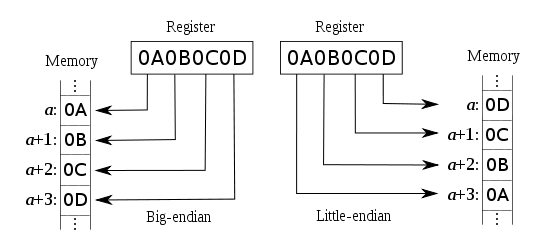
\includegraphics[scale=0.50]{endianess.png}
			\end{center}
			\caption{Diferencias entre \textit{Big Endian} y \textit{Little Endian}}
		\end{figure}
	\end{block}
\end{frame}

\begin{frame}	
\frametitle{Programar para Nintendo Wii}
	\begin{block}{Alineación de los datos}
		\begin{figure}[H]
			\label{alineacion}
			\begin{center}
			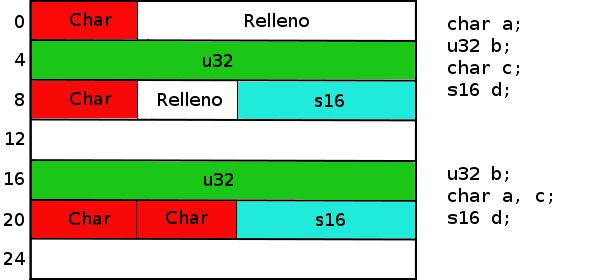
\includegraphics[scale=0.50]{alineacion.png}
			\end{center}
			\caption{Estado de la memoria, alineando o no los datos}
		\end{figure}
	\end{block}
\end{frame}

\begin{frame}	
\frametitle{Programar para Nintendo Wii}
	\begin{block}{Otras consideraciones}
		\begin{itemize}
		\item Alineación y relleno al leer desde un periférico: 32 bytes.
		\item Cantidad de memoria: Wii tiene 64 MB de RAM.
		\item Lanzar un programa: Homebrew Channel.
		\item Tipos de datos.
		\end{itemize}
		\begin{figure}[H]
			\label{tiposdatos}
			\begin{center}
			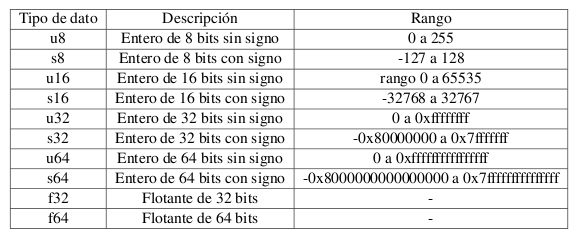
\includegraphics[scale=0.4]{tiposdatos.png}
			\end{center}
			\caption{Tipos de datos utilizados en Nintendo Wii}
		\end{figure}
	\end{block}
\end{frame}

\subsection{Necesidades detectadas}

\begin{frame}	
\frametitle{Necesidades detectadas}
	\begin{block}{Controlar sistemas de la videoconsola}
		\begin{itemize}
			\item Sistema gráfico.
			\begin{itemize}
				\item Dibujo de texturas.
				\item Escritura con fuentes de texto.
			\end{itemize}
			\item Sistema de audio: música y efectos de sonido.
			\item Controladores \textit{Wii Remote}.
			\item Medios de almacenamiento: tarjeta SD.
		\end{itemize}
	\end{block}
	\begin{figure}[H]
		\label{texturas}
		\begin{center}
		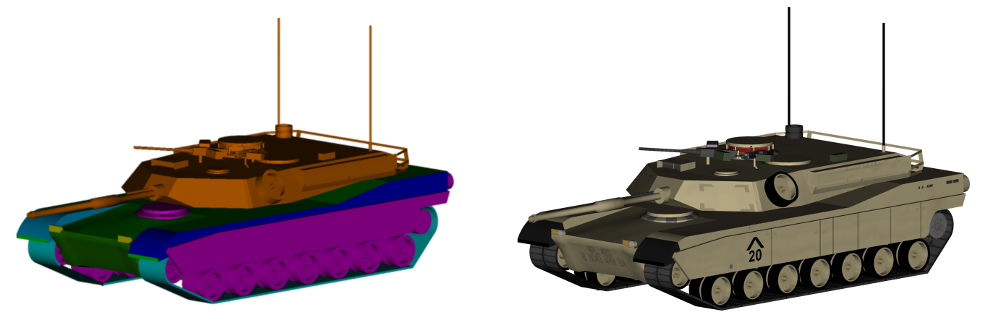
\includegraphics[scale=0.25]{texturas.png}
		\end{center}
		\caption{Figura 3D sin texturas y con texturas}
	\end{figure}
\end{frame}

\begin{frame}	
\frametitle{Necesidades detectadas}
	\begin{block}{Otros módulos con funcionalidad necesaria}
		\begin{itemize}
			\item Analizador XML.
			\item Organizar los recursos multimedia.
			\item Reproducción de animaciones.
			\item Soporte de internacionalización.
			\item Detección de colisiones.
			\item Registro de mensajes del sistema.
		\end{itemize}
	\end{block}
\end{frame}

\begin{frame}	
\frametitle{Necesidades detectadas}
	\begin{block}{Elementos de un juego 2D}
		\begin{itemize}
			\item Actor: elemento con entidad propia dentro del juego.
			\item Escenario: mundo en el que los actores interactúan.
		\end{itemize}
	\end{block}
	\begin{block}{Plantillas}
		\begin{itemize}
			\item Abstraen de los detalles comunes de estos elementos.
			\item Plantilla para actores: base para definir comportamiento.
			\item Plantilla para escenarios: crear niveles de forma sencilla.
			\item Plantilla para clase principal: inicialización de la videoconsola.
		\end{itemize}
	\end{block}
\end{frame}

\begin{frame}	
\frametitle{Necesidades detectadas}
	\begin{block}{Documentación amplia y útil}
		\noindent Facilitar el aprendizaje por medio de documentación.
		\begin{itemize}
			\item Manual de instalación y uso. (34 páginas)
			\item Manual de referencia completo. (Generado con Doxygen)
			\item Memoria del proyecto. (243 páginas)
		\end{itemize}
	\end{block}
	\pause
	\begin{block}{Ejemplos didácticos}
		\noindent Ilustrar el funcionamiento de la biblioteca.
		\begin{itemize}
			\item \textbf{Arkanoid Wii}: romper ladrillos con una bola.
			\item \textbf{Duck Hunt Wii}: cazar patos que aparecen en la pantalla.
			\item \textbf{Wii Pang}: personaje rompe pompas con ganchos verticales.
		\end{itemize}
	\end{block}
\end{frame}

\subsection{Metodología}

\begin{frame}
\frametitle{Metodología}
	\begin{itemize}
		\item Metodología iterativa, basada en \textit{Rational Unified Proccess}.
		\item Por cada etapa se construye un módulo completo.
	\end{itemize}
	\pause
	\begin{block}{Características del sistema}
		\begin{itemize}
			\item Totalmente orientado a objetos.
			\item Separación completa de código fuente y datos: XML.
			\item Fase de diseño:
			\begin{itemize}
				\item Patrón \textit{Singleton}: para los módulos con una única instancia.
				\item Patrón Visitante: para la implementación de \textit{Double Dispatch} en el módulo de colisiones.
			\end{itemize}
		\end{itemize}
	\end{block}
\end{frame}

\subsection{Detalles de implementación}

\begin{frame}
\frametitle{Detalles de implementación}
	\begin{block}{Proyección ortográfica}
		\begin{itemize}
			\item Foco de luz en el infinito.
			\item Proyectar perpendicularmente a la pantalla.
			\item No hay cambios de tamaño por distancia al plano.
		\end{itemize}
	\end{block}
	\begin{figure}[H]
		\label{ortho}
		\begin{center}
		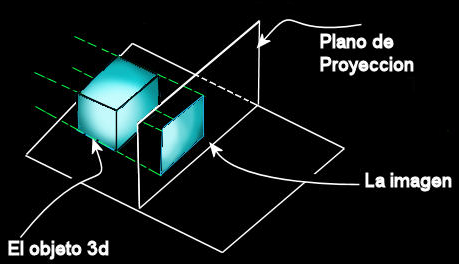
\includegraphics[scale=0.4]{ortho.png}
		\end{center}
		\caption{Proyección ortográfica}
	\end{figure}
\end{frame}

\begin{frame}
\frametitle{Detalles de implementación}
	\begin{block}{Doble búfer}
		\begin{itemize}
			\item Dos zonas de memoria para dibujar fotogramas.
			\item Se consigue evitar parpadeos al mostrar animaciones.
		\end{itemize}
	\end{block}
	\begin{figure}[H]
		\label{doblebuffer}
		\begin{center}
		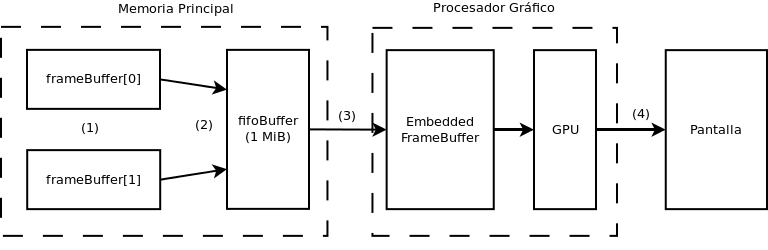
\includegraphics[scale=0.4]{doblebuffer.png}
		\end{center}
		\caption{Esquema del sistema gráfico con doble búfer}
	\end{figure}
\end{frame}

\begin{frame}
\frametitle{Detalles de implementación}
	\begin{block}{Formato de vídeo RGB5A3}
		\begin{itemize}
		\item Formato nativo con el que trabaja el procesador gráfico.
		\item Permite trabajar cómodamente con transparencias.
		\end{itemize}
	\end{block}
	\begin{figure}[H]
		\label{rgb5a3}
		\begin{center}
		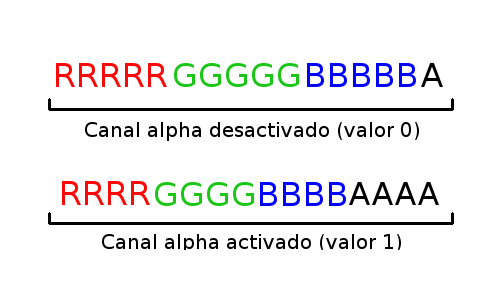
\includegraphics[scale=0.45]{rgb5a3.png}
		\end{center}
		\caption{Formato de píxel RGB5A3}
	\end{figure}
\end{frame}

\begin{frame}
\frametitle{Detalles de implementación}
	\begin{block}{Texturas organizadas en \textit{tiles}}
		\begin{itemize}
			\item Píxeles adyacentes en la imagen, también en memoria.
			\item GPU usa texturas en tiles para trabajar de forma optimizada.
		\end{itemize}
	\end{block}
	\begin{figure}[H]
		\label{texturatiles}
		\begin{center}
		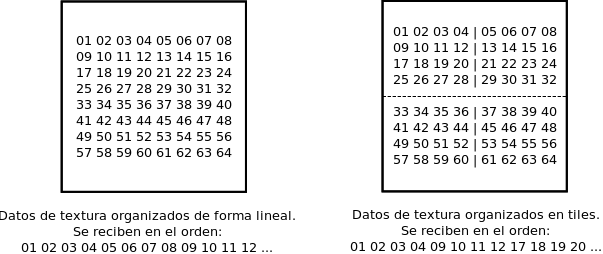
\includegraphics[scale=0.45]{texturatiles.png}
		\end{center}
		\caption{Textura lineal y textura organizada en \textit{tiles} de 4x4}
	\end{figure}
\end{frame}

\begin{frame}
\frametitle{Detalles de implementación}
	\begin{block}{Sistema de audio}
		\begin{itemize}
		\item Procesador DSP dedicado únicamente al control de audio.
		\item Reproduce hasta 16 flujos de sonido (voces) simultáneamente.
		\item Una voz reservada para pistas de música.
		\item Formato nativo de Wii:
			\begin{itemize}
			\item 48000 Hz.
			\item Estéreo (dos canales).
			\item \textit{Samples} de 16 bits con signo.
			\end{itemize}
		\end{itemize}
	\end{block}
\end{frame}

\begin{frame}
\frametitle{Detalles de implementación}
	\begin{block}{Fuentes de texto}
		\begin{itemize}
		\item \textit{FreeType2} genera una imagen \textit{bitmap} para cada carácter.
		\item Mapa de bits monocromo: un píxel se dibuja si tiene valor 1.
		\item En pantalla se dibuja cada carácter píxel a píxel.
		\end{itemize}
	\end{block}
	\begin{figure}[H]
		\label{fuentestexto}
		\begin{center}
		
\includegraphics[scale=0.45]{fuentestexto.png}
		\end{center}
		\caption{Mapa de bits monocromo asociado al caracter \textit{a}}
	\end{figure}
\end{frame}

\begin{frame}
\frametitle{Detalles de implementación}
	\begin{block}{Colisiones: Técnica de \textit{Double Dispatch}}
		\noindent Evita tener que identificar el tipo de dos objetos derivados de la misma clase base.
	\end{block}
	\begin{figure}[H]
		\label{doubledispatch}
		\begin{center}
		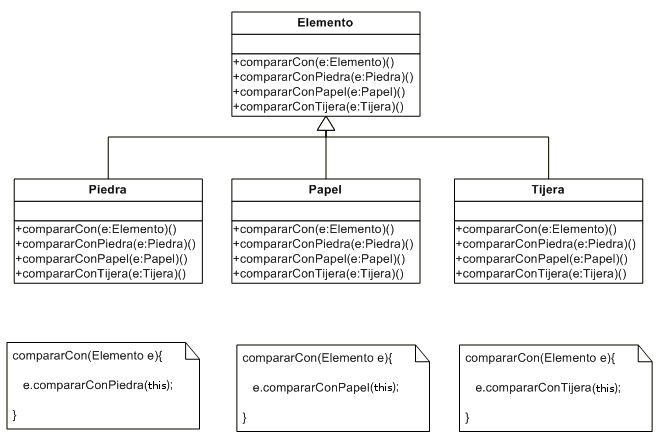
\includegraphics[scale=0.40]{doubledispatch.png}
		\end{center}
	\end{figure}
\end{frame}

\begin{frame}
\frametitle{Detalles de implementación}
	\begin{block}{Escenarios: Mapas de \textit{tiles}}
		\noindent \textbf{Tile}: una imagen cuadrada, rectangular o hexagonal, utilizada para generar imágenes de mayor complejidad.
	\end{block}
	\begin{figure}[H]
		\label{tileset}
		\begin{center}
		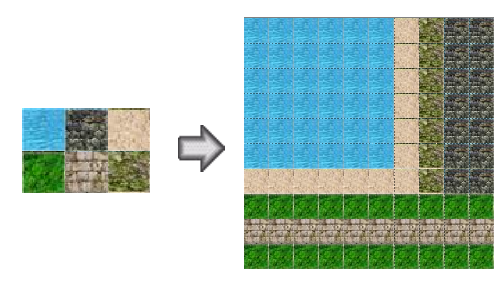
\includegraphics[scale=0.4]{tileset.png}
		\end{center}
		\caption{\textit{Tileset} (conjunto de \textit{tiles}) y mapa de \textit{tiles}}
	\end{figure}
\end{frame}

\subsection{Herramientas utilizadas}

\begin{frame}
\frametitle{Herramientas utilizadas}
	\begin{block}{Tecnología}
		\begin{itemize}
			\item C++, con GNU Make.
			\item XML
		\end{itemize}
	\end{block}
	\begin{block}{Desarrollo}
		\begin{itemize}
			\item \textbf{Gimp}: edición de imágenes.
			\item \textbf{SoX}: edición de sonido.
			\item \textbf{Doxygen}: documentación automática de código.
			\item \textbf{\LaTeX}: sistema de composición de textos.
			\item \textbf{Gantt Project}: diagramas de planificación.
			\item \textbf{Dia}: editor de diagramas UML.
			\item \textbf{Cppcheck}: analizador estático de código fuente C++.
			\item \textbf{Subversion}: control de revisiones.
			\item \textbf{Tiled}: editor de mapas de \textit{tiles}.
		\end{itemize}
	\end{block}
\end{frame}

\begin{frame}
\frametitle{Herramientas utilizadas}
	\begin{block}{DevKitPPC}
		\begin{itemize}
			\item Generación de ejecutables para sistemas \textit{Power PC}.
			\item Reglas de compilación específicas para Wii.
			\item Fácilmente ampliable con bibliotecas externas.
			\item \textbf{Wiiload}: lanzar ejecutables mediante red local.
		\end{itemize}
	\end{block}
	\begin{block}{Bibliotecas externas}
		\noindent Previamente adaptadas para trabajar con \textit{DevKitPPC}.
		\begin{itemize}
			\item \textbf{Libogc}: permite acceder al hardware de Nintendo Wii.
			\item \textbf{Libfat}: para trabajar con particiones FAT/FAT32
			\item \textbf{FreeType2}: necesaria para utilizar fuentes de texto.
			\item \textbf{TinyXml}: proporciona una interfaz para trabajar con XML.
		\end{itemize}
	\end{block}
\end{frame}

\subsection{Pruebas y validación}

\begin{frame}
\frametitle{Pruebas y validación}
	\begin{block}{Especificación de las pruebas}
		\begin{itemize}
			\item Garantizar el buen funcionamiento de la herramienta.
			\item Se han realizado durante y después del desarrollo.
			\item Han consistido en varios grupos de pruebas:
			\begin{itemize}
				\item Pruebas de módulo.
				\item Pruebas de sistema.
				\item Pruebas de \textit{makefile}.
				\item Pruebas de juegos.
				\item Análisis estático del código con \textit{Cppcheck}.
			\end{itemize}
			\item Todas las pruebas se han realizado sobre la videoconsola.
		\end{itemize}
	\end{block}
\end{frame}

\begin{frame}
\frametitle{Pruebas y validación}
	\begin{block}{Pruebas de módulo}
		\noindent Prueba exhaustiva de cada módulo, tras finalizar su desarrollo:
		\begin{itemize}
			\item Caja blanca: comprobar los distintos caminos que toma el flujo de ejecución en el módulo.
			\item Caja negra: partiendo de conjuntos de datos de entrada y comprobando la salida que producen.
		\end{itemize}
	\end{block}
	\pause
	\begin{block}{Pruebas de sistema}
		\noindent Comprobar funcionamiento de cada módulo junto con los demás.
		\begin{itemize}
			\item Animación e Imagen.
			\item Galería y recursos multimedia.
			\item Actor y figuras de colisión.
			\item Etc.
		\end{itemize}
	\end{block}
\end{frame}

\begin{frame}[fragile]
\frametitle{Pruebas y validación}
	\begin{block}{Pruebas de \textit{makefile}}
		\begin{itemize}
			\item Compilación.
			\item Generación de documentación.
			\item Empaquetado.
			\item Instalación y desinstalación.
		\end{itemize}
	\end{block}
	\begin{block}{Pruebas de juegos}
		\begin{itemize}
			\item \textit{Playtesting}: varias personas juegan y reportan errores.
		\end{itemize}
	\end{block}
	\begin{block}{Análisis estático de código fuente}
		\begin{itemize}
			\item Se utilizó Cppcheck.
			\item \begin{lstlisting}{style=C, frame=none}
				> cppcheck --enable=all include src
			\end{lstlisting}
		\end{itemize}
	\end{block}
\end{frame}

\begin{frame}
\frametitle{Pruebas y validación}
	\begin{block}{Problemas surgidos durante el desarrollo}
		\begin{itemize}
			\item Poca documentación existente: tutoriales muy incompletos.
			\item Control de la eficiencia: hardware limitado.
			\item Trabajo a bajo nivel con recursos: imágenes y fuentes.
			\item Difícil depuración.
		\end{itemize}
	\end{block}
	\begin{figure}[H]
		\label{excepcion}
		\begin{center}
		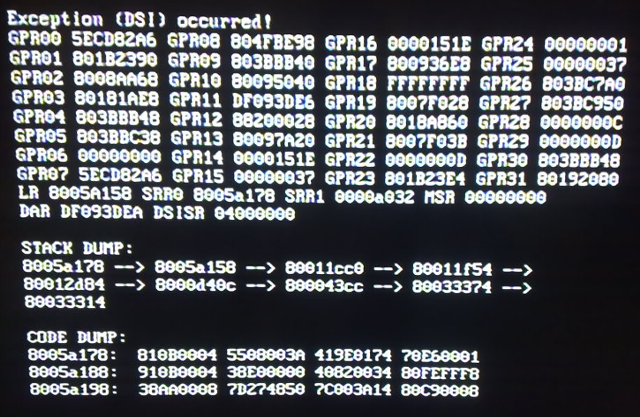
\includegraphics[scale=0.3]{excepcion.png}
		\end{center}
	\end{figure}
\end{frame}


% Conclusiones
% Este archivo es parte de la presentación de libWiiEsp, protegida bajo la 
% licencia GFDL. Copyright (C) 2011 Ezequiel Vázquez de la Calle

% -*-conclusiones.tex-*-

\section{Conclusiones}

\begin{frame}	
\frametitle{Conclusiones}
	\begin{block}{Cumplimiento de objetivos}
		\begin{itemize}
			\item Se da acceso a los subsistemas de Nintendo Wii.
			\item Se cubren los puntos básicos de videojuegos 2D:
			\begin{itemize}
				\item Gestión de recursos multimedia.
				\item Animaciones.
				\item Detección de colisiones.
				\item Soporte de internacionalización.
				\item Diseño de escenarios.
				\item Registro de mensajes del sistema.
			\end{itemize}
			\item Documentación completa, útil y en español.
			\item Tres juegos de ejemplo.
			\begin{itemize}
				\item Mecánicas diferentes.
				\item Código fuente totalmente comentado.
			\end{itemize}
		\end{itemize}
	\end{block}
\end{frame}

\begin{frame}	
\frametitle{Conclusiones}
	\begin{block}{Objetivos personales}
		\begin{itemize}
			\item Desarrollo de biblioteca partiendo de una base pequeña.
			\item Aprendizaje de varias herramientas libres:
			\begin{itemize}
				\item Profundización en GNU Make.
				\item Bibliotecas: Libfat, FreeType2 y TinyXML.
				\item Doxygen.
				\item \LaTeX.
				\item Subversion.
			\end{itemize}
			\item Adquisición de conocimientos sobre Nintendo Wii:
			\begin{itemize}
				\item Trabajo con formatos multimedia.
				\item Control de los mandos de la videoconsola.
				\item Comprender cómo funciona Wii internamente.
			\end{itemize}
			\item Puesta en práctica de los conocimientos adquiridos.
			\item Contribución al mundo del Software Libre y el \textit{Homebrew}.
		\end{itemize}
	\end{block}
\end{frame}

\begin{frame}	
\frametitle{Conclusiones}
	\begin{block}{Posibles mejoras}
		\begin{itemize}
			\item Sistema de sonido 3D.
			\item Soporte para otros periféricos de Nintendo Wii.
			\item Puertos USB traseros.
		\end{itemize}
	\end{block}
	\begin{block}{Futuro del proyecto}
		\begin{itemize}
			\item Desarrollo de juegos más complejos.
			\item Creación de comunidad de desarrolladores.
		\end{itemize}
	\end{block}
\end{frame}


% Bibliografia
% Este archivo es parte de la presentación de libWiiEsp, protegida bajo la 
% licencia GFDL. Copyright (C) 2011 Ezequiel Vázquez de la Calle

% -*-bibliografia.tex-*-

\section{Bibliografía y referencias}

\begin{frame}
\frametitle{Bibliografía recomendada}
\begin{thebibliography}{5}
\beamertemplatearticlebibitems
	\bibitem{DevKitPro}
	Página oficial del proyecto DevKitPro.
	\newblock http://www.devkitpro.org
	
	\bibitem{WiiBrew}
	Wiki sobre \textit{homebrew} para Nintendo Wii.
	\newblock http://www.wiibrew.org
	
	\bibitem{Hermes}
	Tutorial de programación para Nintendo Wii (Hermes).
	\newblock http://www.elotrolado.net/wiki/Curso\_de\_programacion

	\bibitem{SceneBeta}
	Tutoriales de programación para Nintendo Wii de Scene Beta.
	\newblock http://wii.scenebeta.com/tutoriales/wii
	 
\beamertemplatebookbibitems
	\bibitem{C++}
	Aburruzaga García, Medina Bulo, Palomo Lozano
	\newblock Fundamentos de C++. Servicio de Publicaciones UCA, 2001. ISBN: 84-7786-734-8.
\end{thebibliography}
\end{frame}

\begin{frame}
\frametitle{Demostración}
\begin{center}
	{\LARGE Demostración de los juegos de ejemplo}\\
	\bigskip
	{\large Arkanoid Wii}\\
	\medskip
	{\large Wii Pang}\\
	\medskip
	{\large Duck Hunt Wii}
\end{center}
\end{frame}

\begin{frame}
\frametitle{Esto es todo...}
\begin{center}
	{\LARGE Gracias por su atención}\\
	\medskip
	{\large ¿Preguntas?}\\
	\bigskip
	http://libwiiesp.forja.rediris.es/
\end{center}
\end{frame}


\end{document}

